\section{Usage Examples}

Below are some examples of interaction with the application, illustrating the main usage flows.

Specifically, the following use cases are shown:

\begin{itemize}
  \item \textbf{Explore the platform}
  \item \textbf{Login and Registration}
  \item \textbf{Create an event}
  \item \textbf{Attend an event}
  \item \textbf{Review an event}
  \item \textbf{Contact an organization}
\end{itemize}

The storyboards are presented directly using the developed platform, showing the main user interactions.

In the examples below, some secondary or repetitive navigation dynamics have been omitted.

\subsection{Explore the Platform}

A user who opens the platform can start exploring it. In particular, they can discover proposed events or search for them directly via the search bar. If they want to see more results, they can go to a dedicated page for exploring the platform content, where it is possible to filter events and more conveniently search for users and organizations.

\begin{figure}[H]
  \centering
  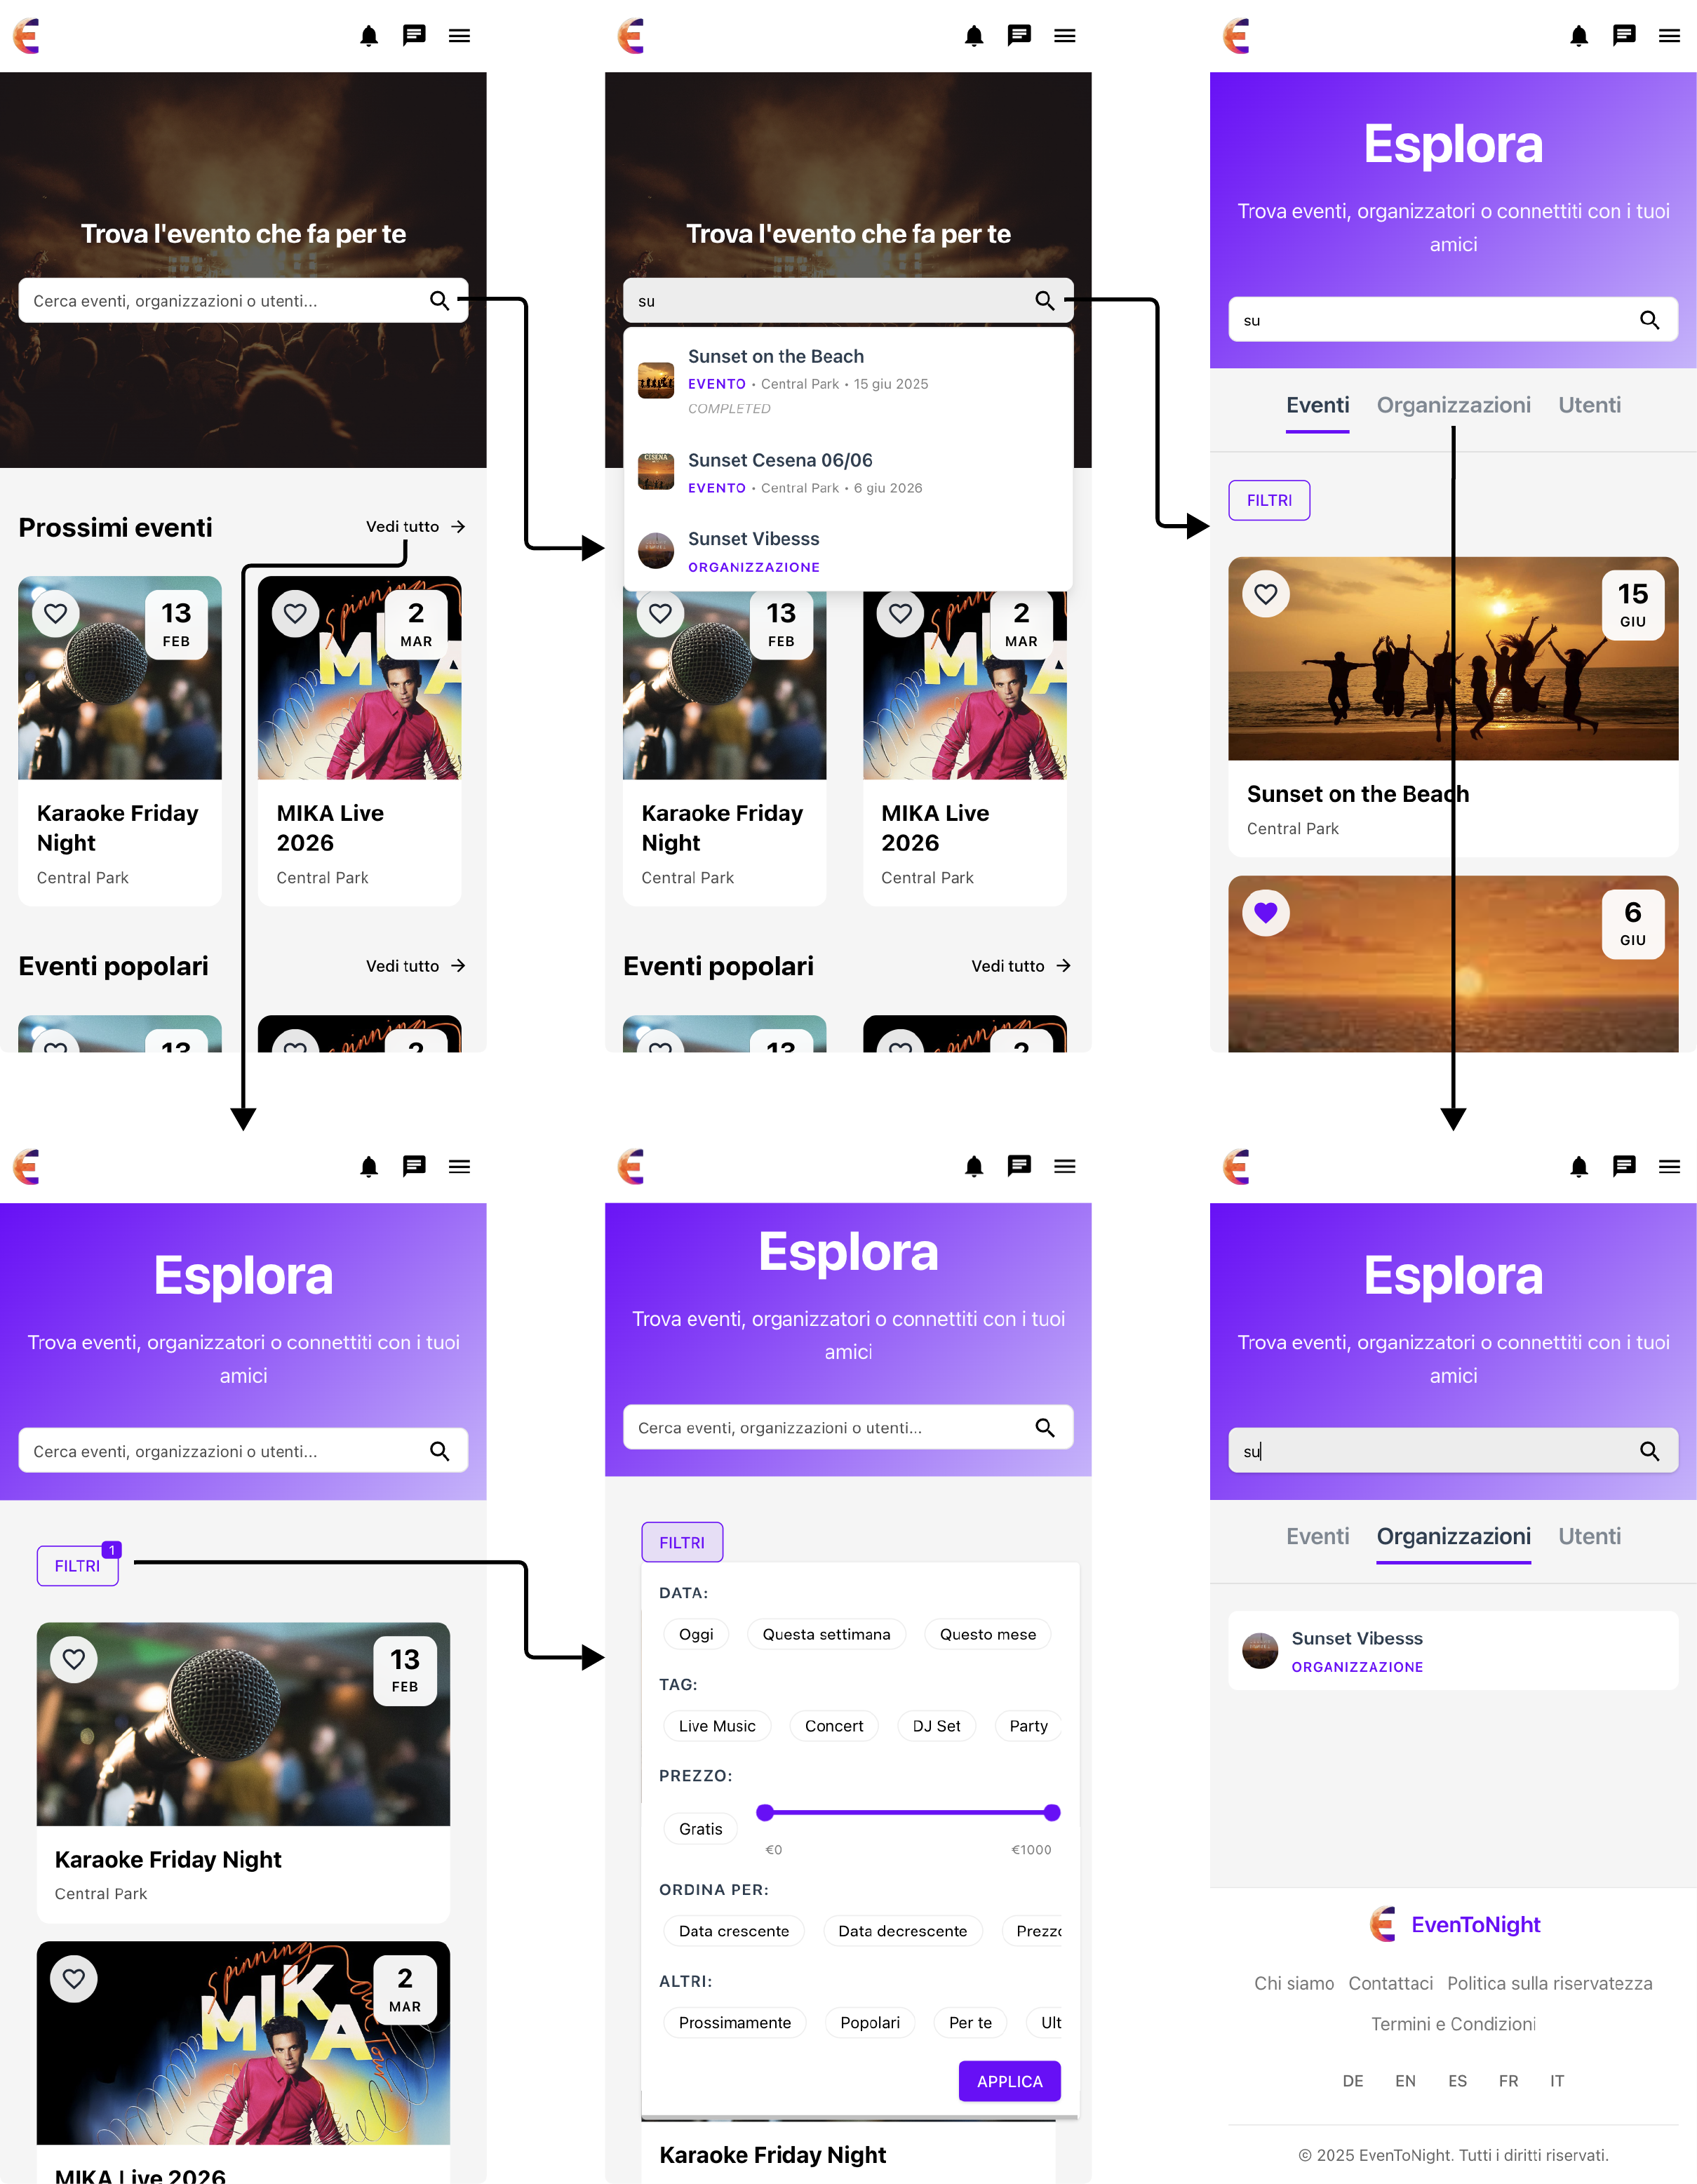
\includegraphics[width=\textwidth]{../public/storyboard/Storyboard-Explore.png}
  \caption{Storyboard: Exploring the platform}
  \label{fig:storyboard-explore}
\end{figure}

\subsection{Login and Registration}

After opening the application, a user can log in or register to access the additional features offered by the platform.

\begin{figure}[H]
  \centering
  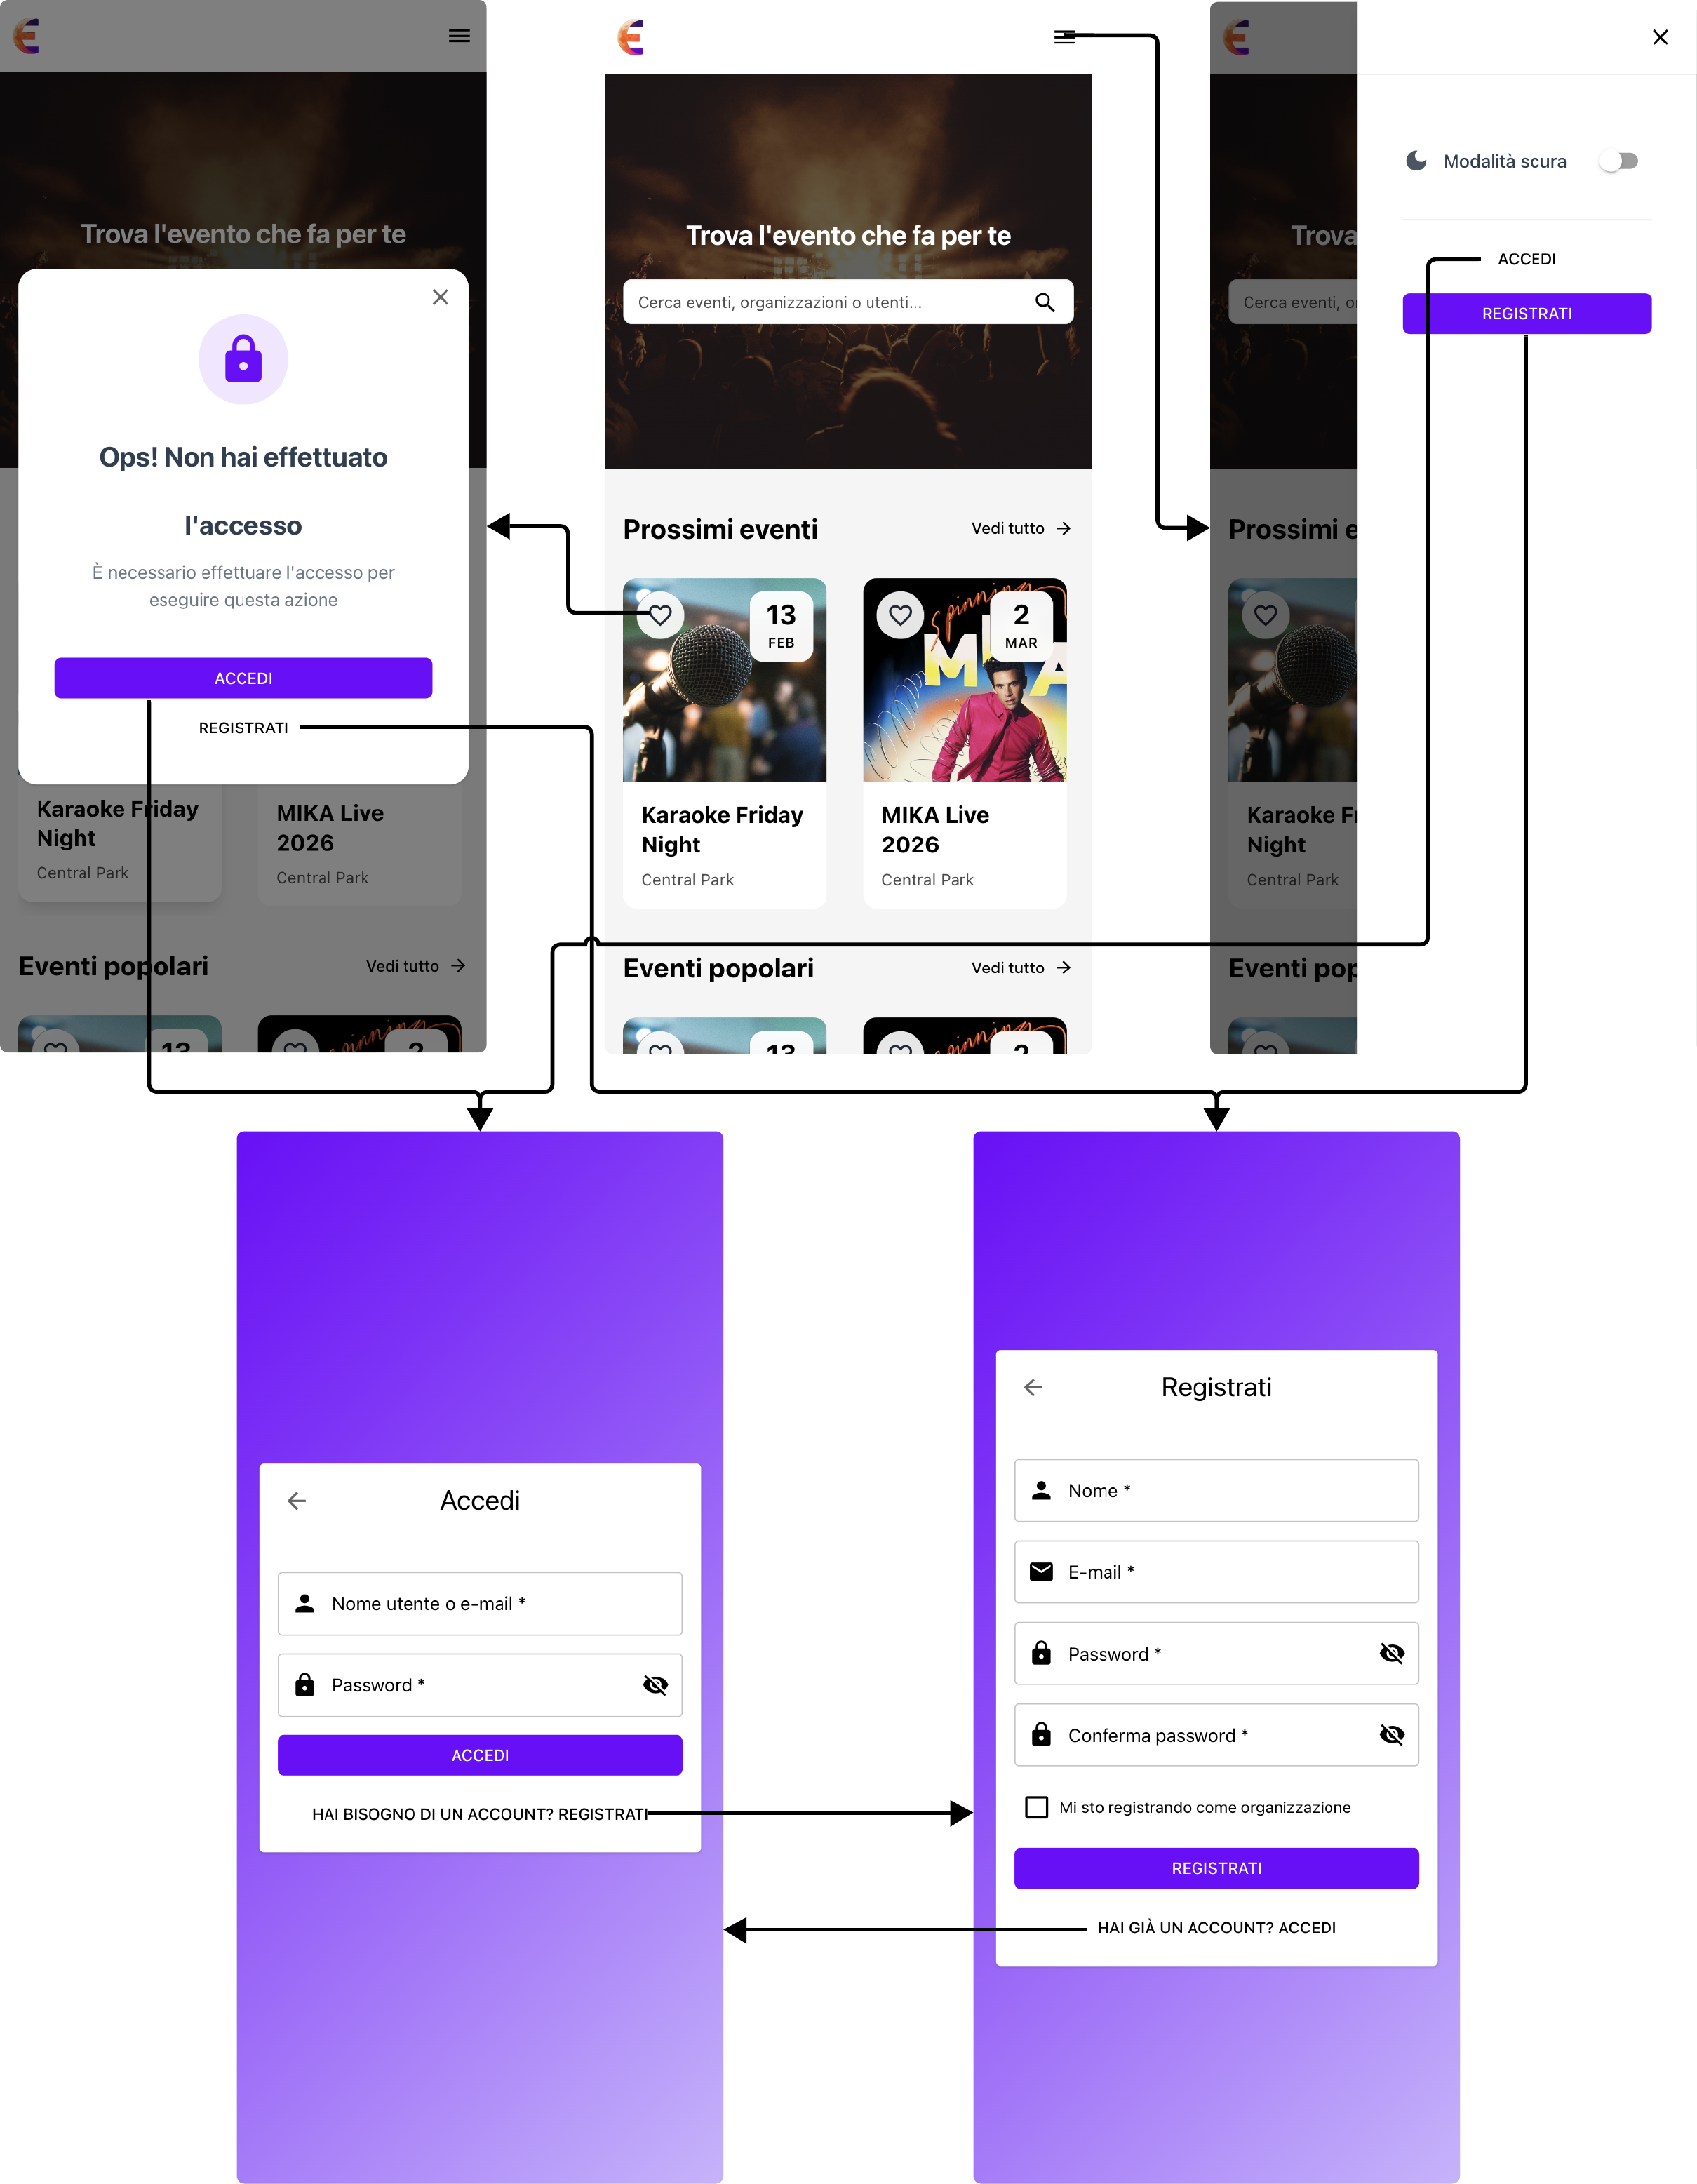
\includegraphics[width=\textwidth]{../public/storyboard/Storyboard-Login.png}
  \caption{Storyboard: Login and registration}
  \label{fig:storyboard-login}
\end{figure}

\subsection{Create an Event}

An organization that has registered on the platform can create events. The creation happens through a form where all the relevant data is entered. It is also possible to temporarily create a draft of the event and continue editing it later.

\begin{figure}[H]
  \centering
  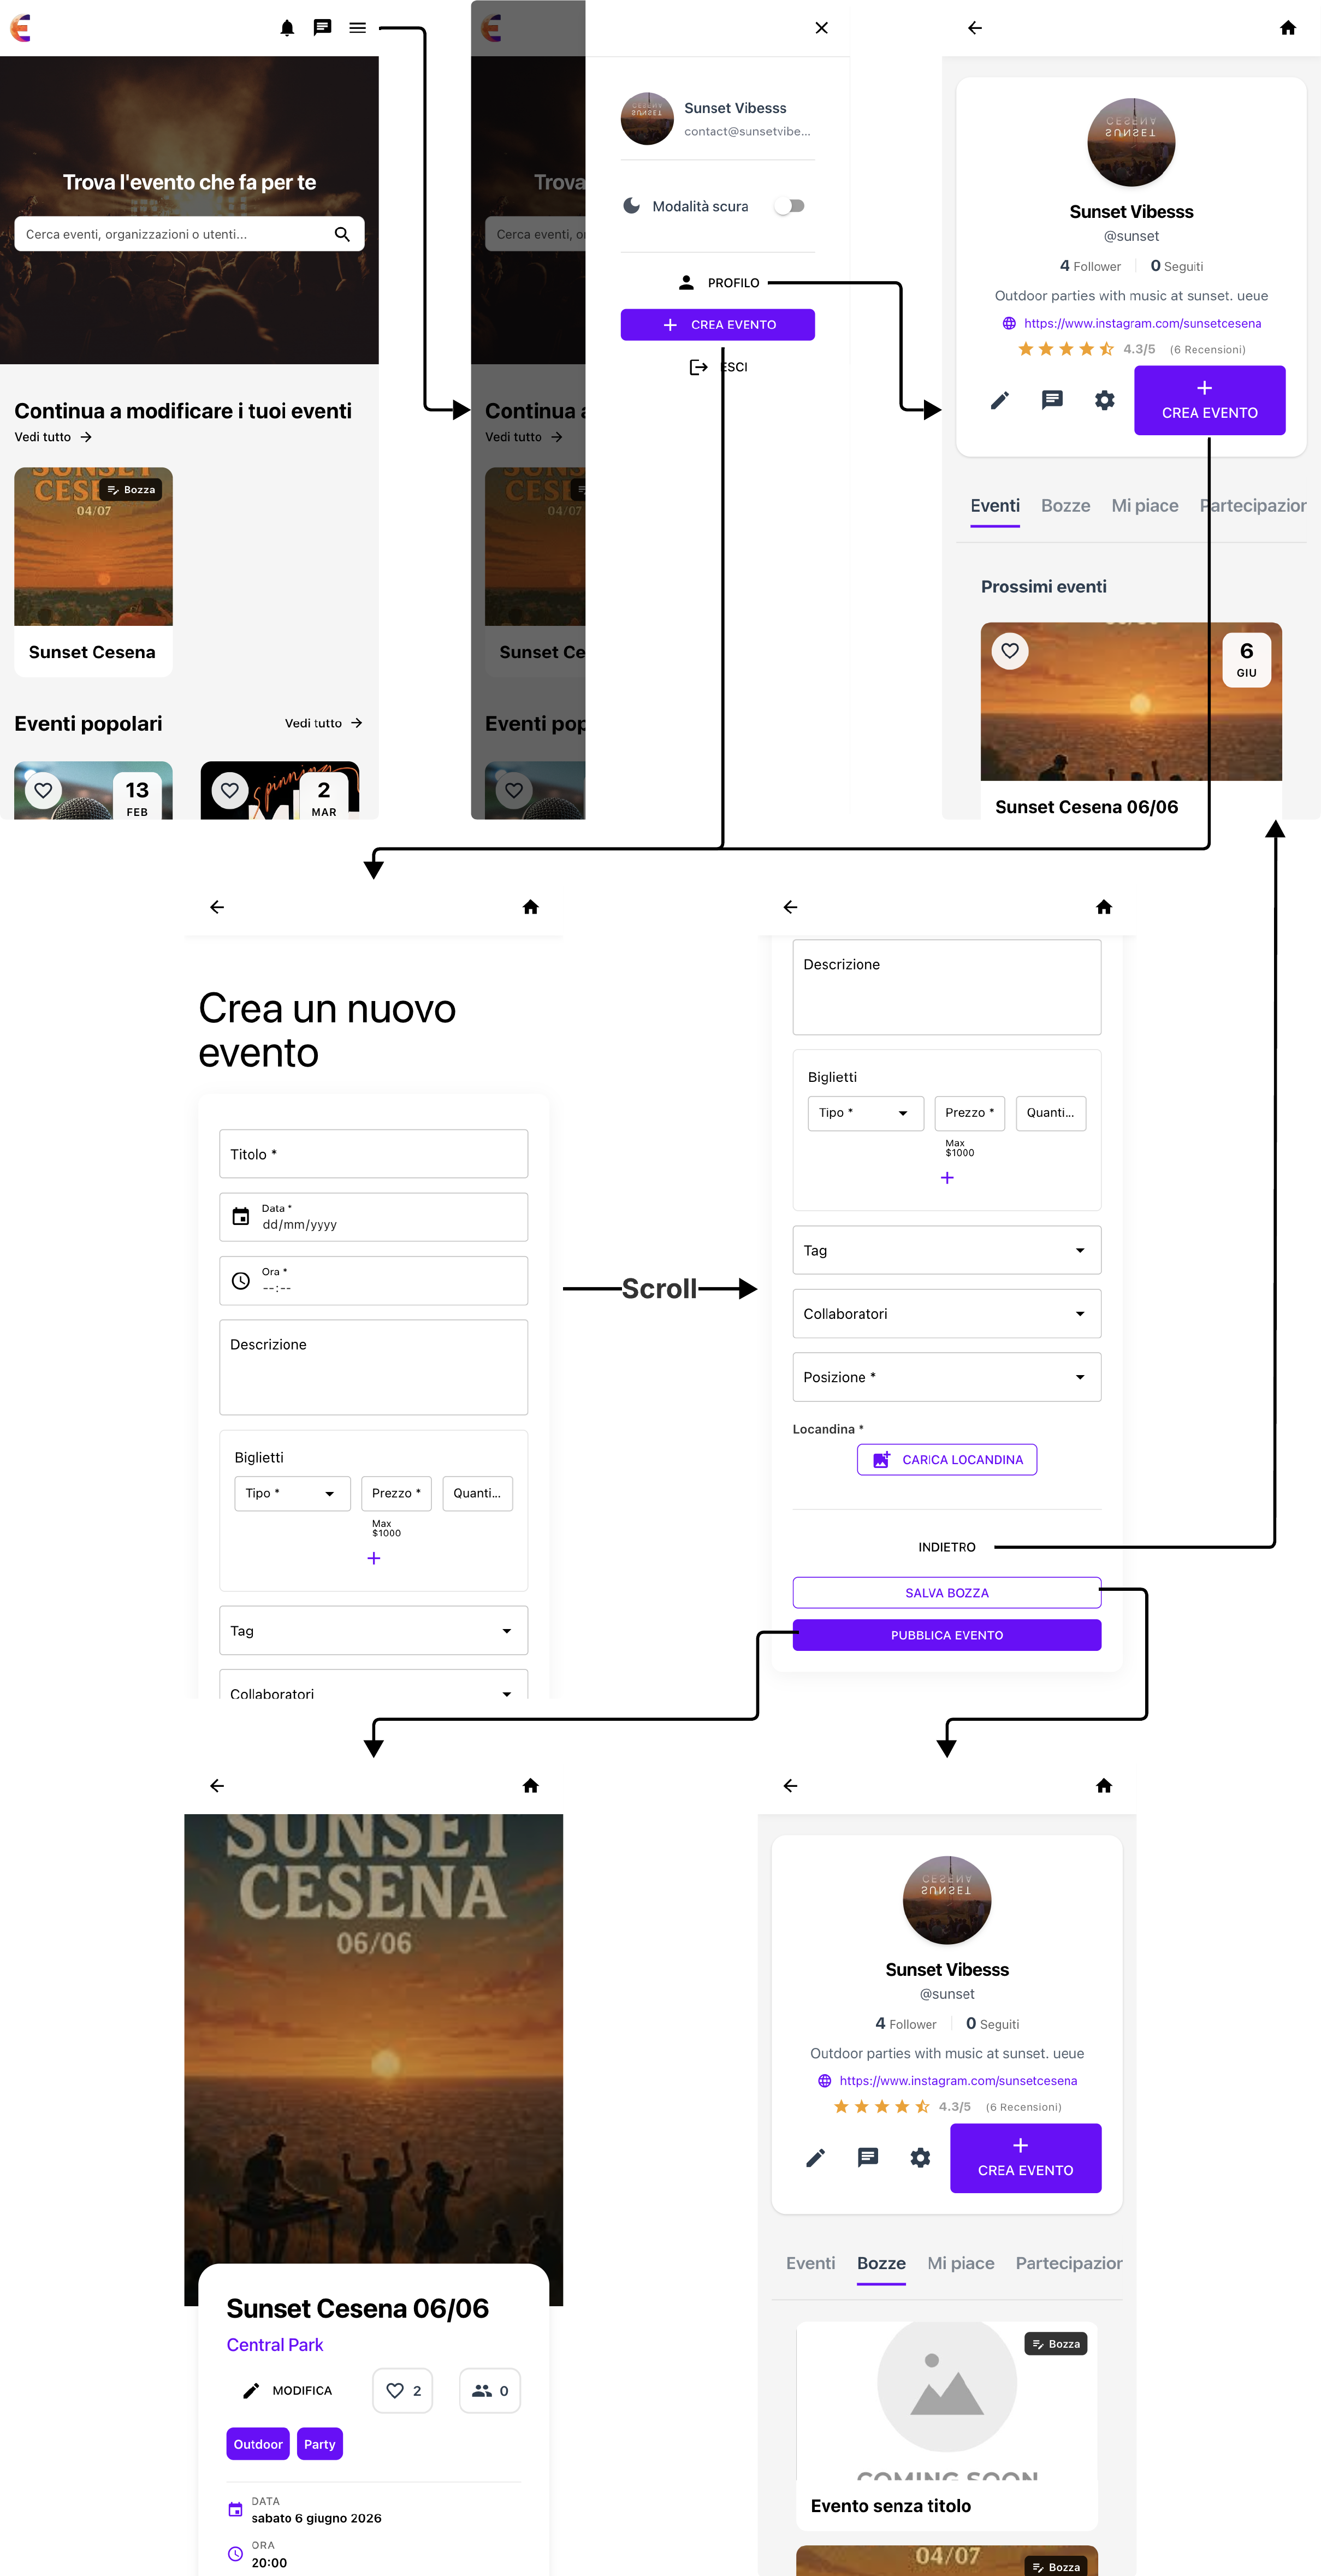
\includegraphics[width=0.75\textwidth]{../public/storyboard/Storyboard-Create-Event.png}
  \caption{Storyboard: Creating an event}
  \label{fig:storyboard-create-event}
\end{figure}

\subsection{Attend an Event}

A registered user can purchase tickets for different events and view them later. The tickets will contain a QR code that organizations can use to verify them.

\begin{figure}[H]
  \centering
  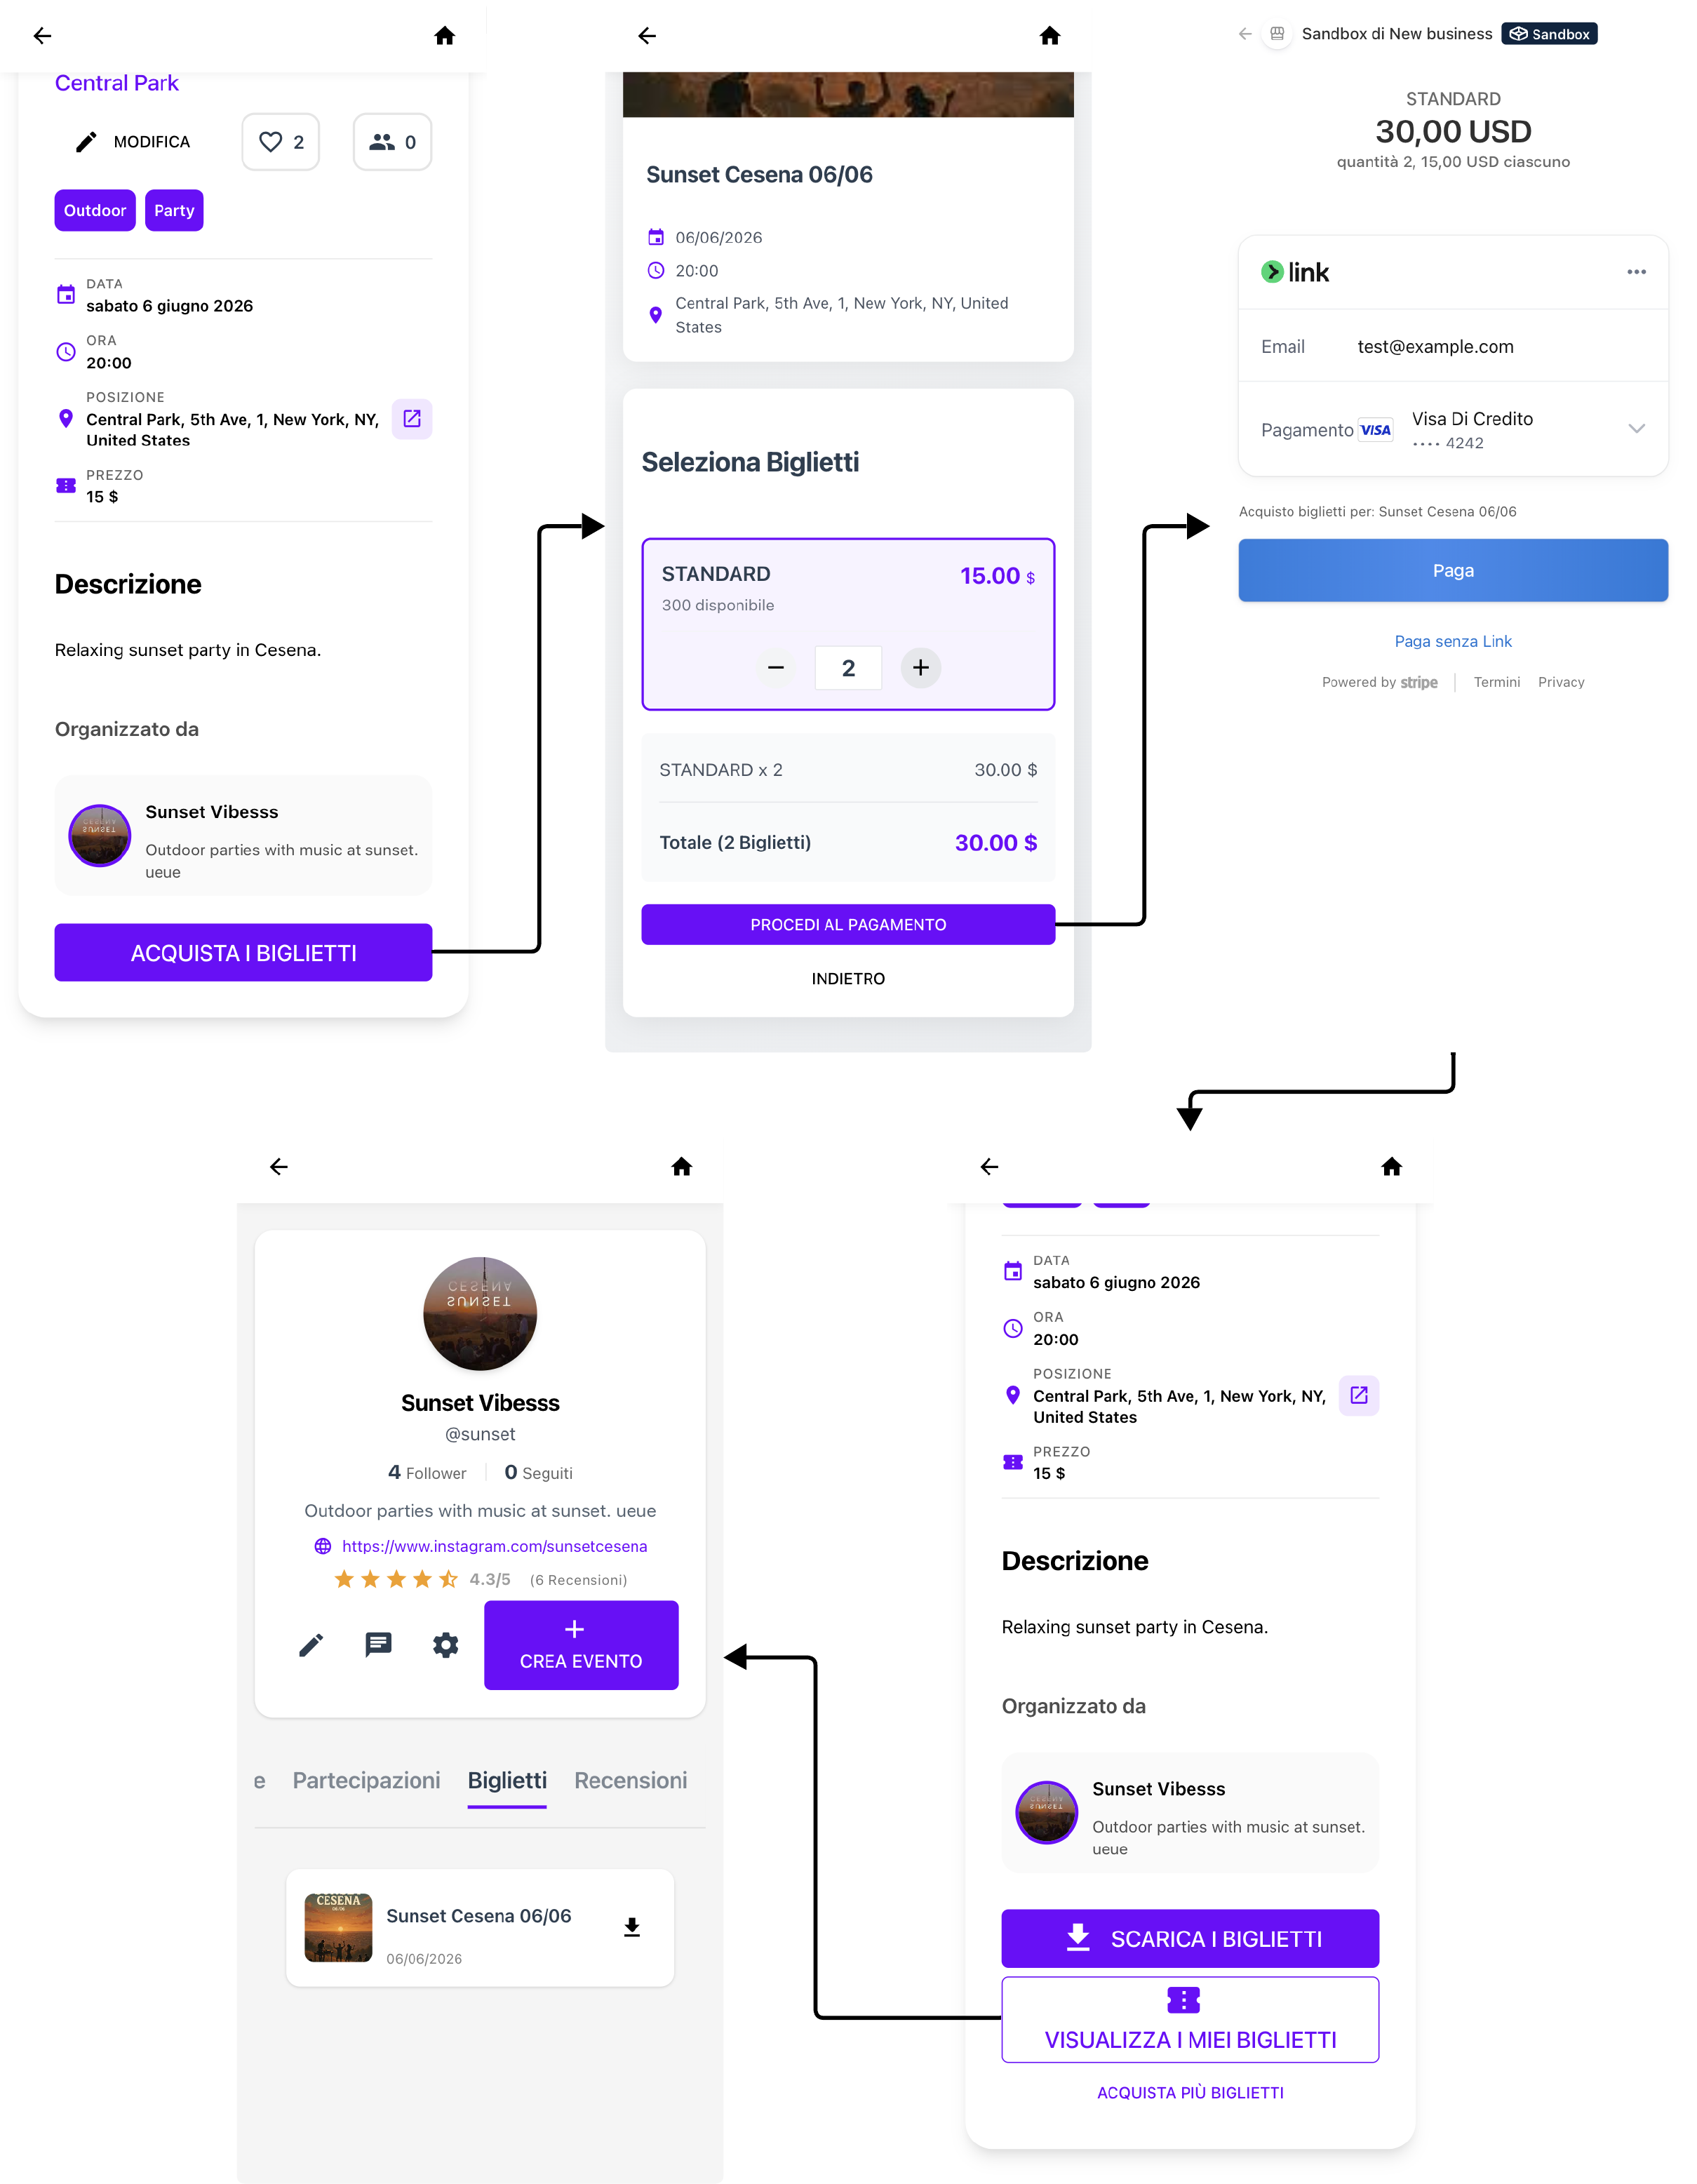
\includegraphics[width=\textwidth]{../public/storyboard/Storyboard-Buy-Ticket.png}
  \caption{Storyboard: Purchasing a ticket}
  \label{fig:storyboard-buy-ticket}
\end{figure}

\subsection{Review an Event}

After attending an event, a user can decide to leave a review. Once submitted, they cannot leave another review for the same event, but they can modify or delete it.

\begin{figure}[H]
  \centering
  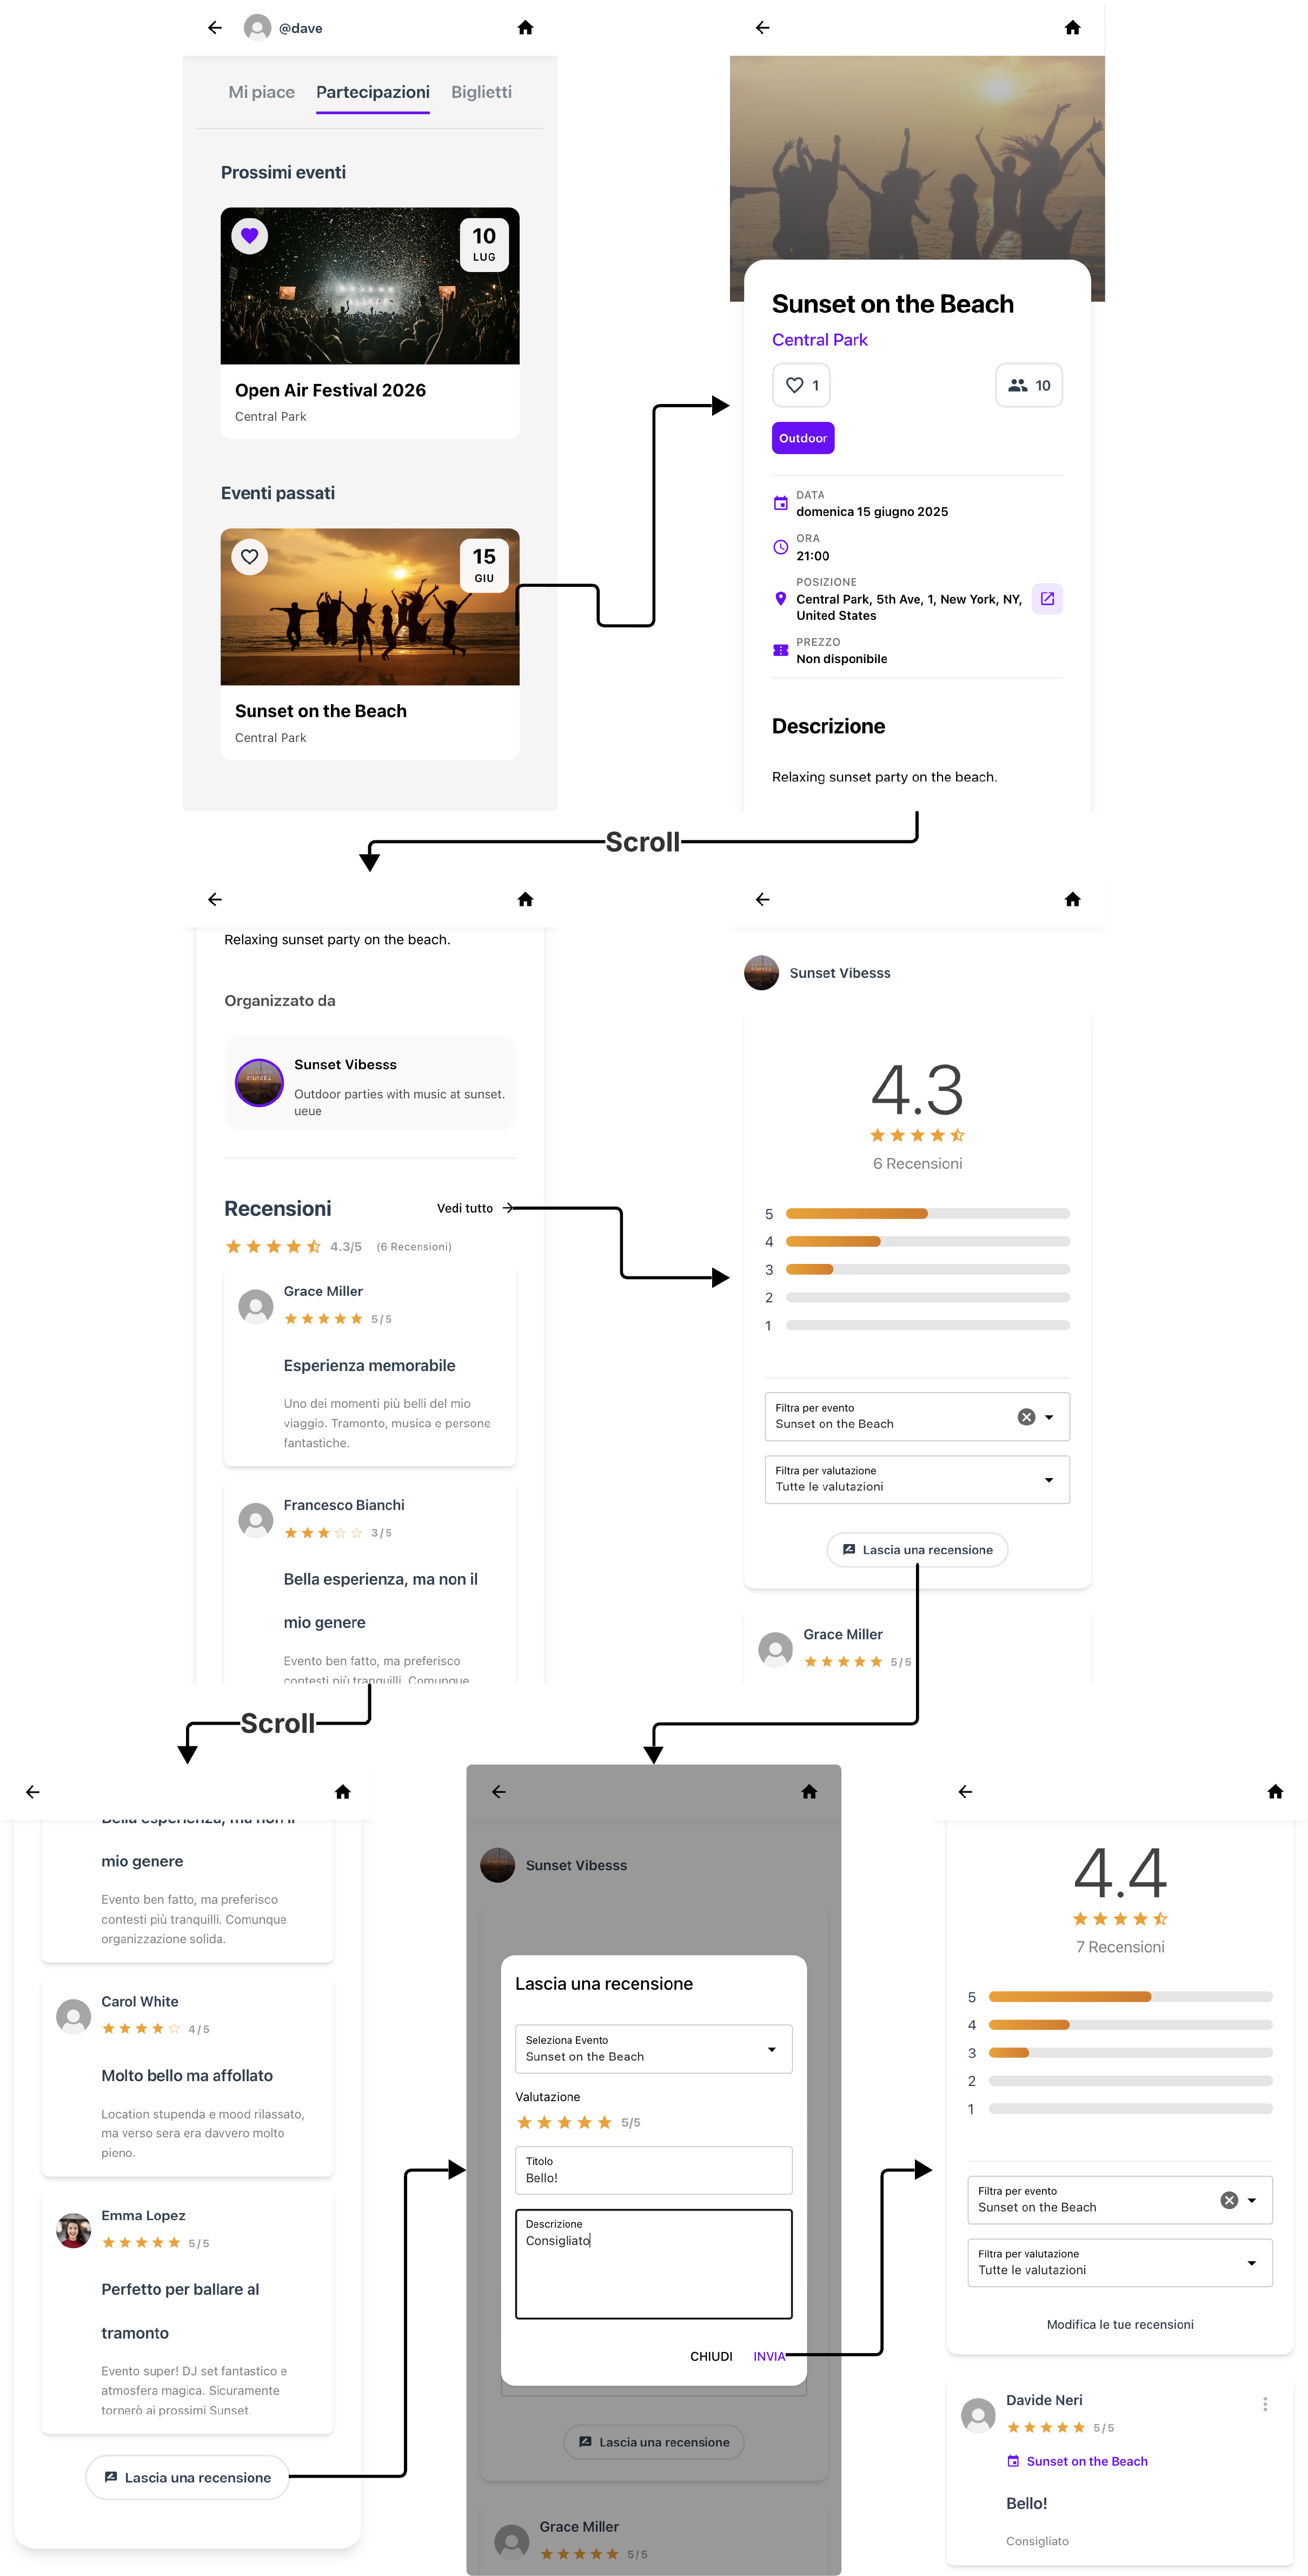
\includegraphics[width=0.65\textwidth]{../public/storyboard/Storyboard-Reviews.png}
  \caption{Storyboard: Reviewing an event}
  \label{fig:storyboard-reviews}
\end{figure}

\subsection{Contact an Organization}

A registered user may need to contact an organization to ask for more information or for potential issues.

\begin{figure}[H]
  \centering
  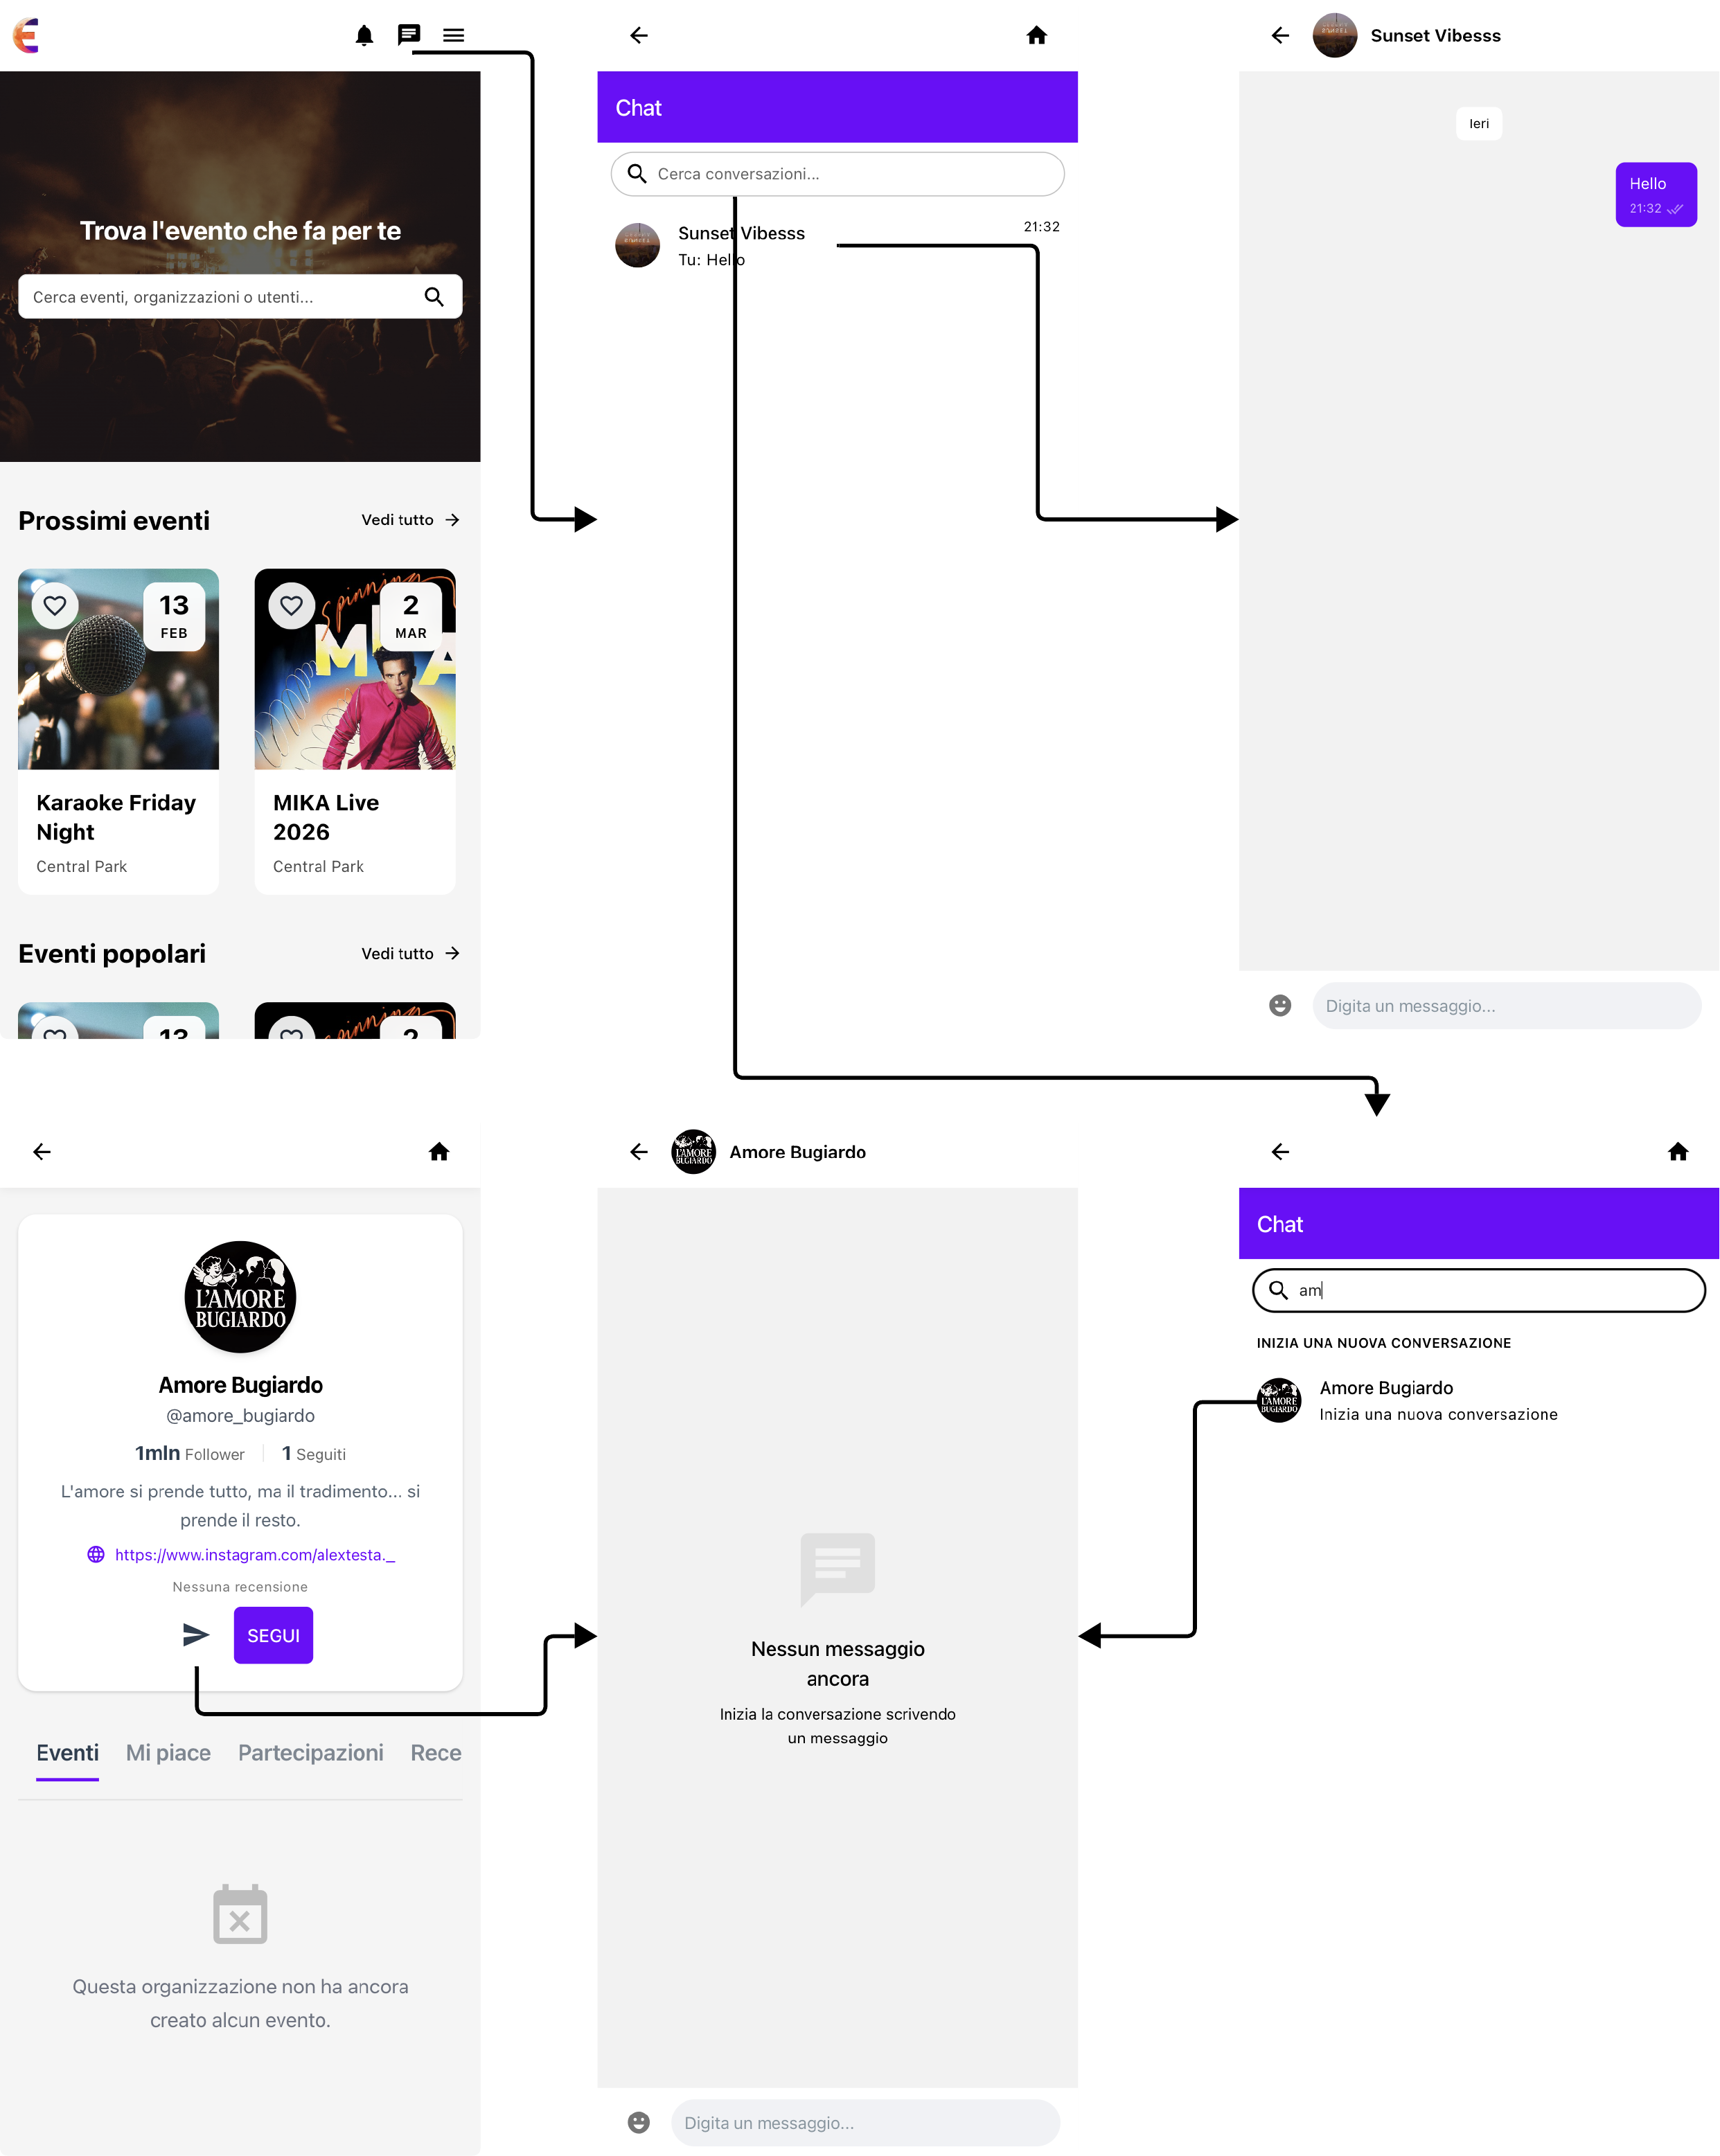
\includegraphics[width=\textwidth]{../public/storyboard/Storyboard-Chat.png}
  \caption{Storyboard: Contacting an organization}
  \label{fig:storyboard-chat}
\end{figure}
